\documentclass{standalone}
\usepackage{tikz}
\usetikzlibrary{patterns, positioning}
\usepackage[sfdefault]{ClearSans} %% option 'sfdefault' activates Clear Sans as the default text font
\usepackage[T1]{fontenc}

\begin{document}
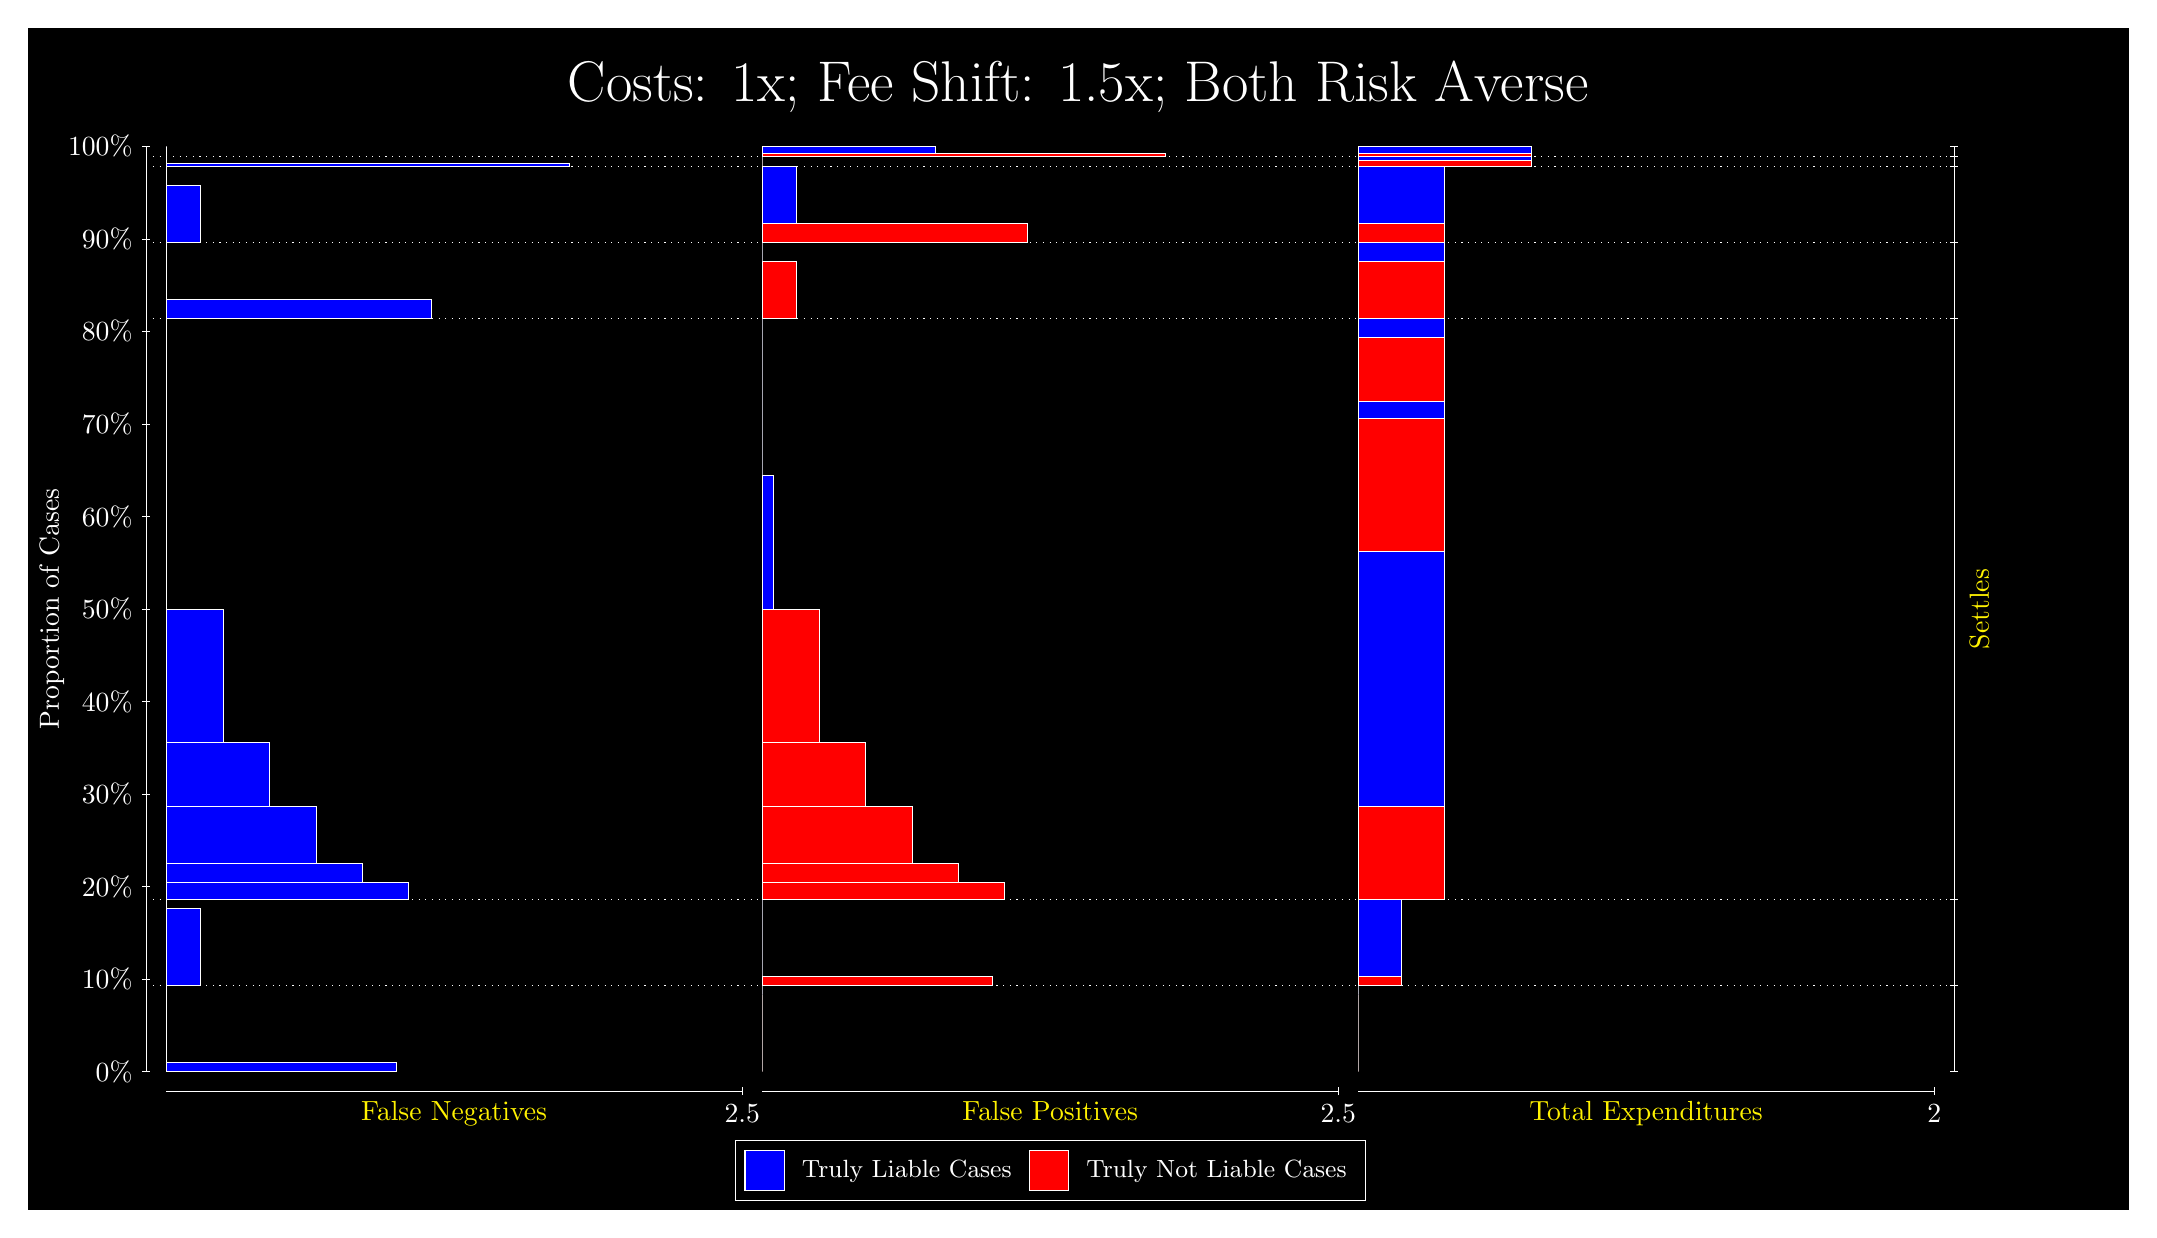
\begin{tikzpicture}
\draw[fill=black] (0,0) rectangle (26.667,15);
\draw[text=white] (0,13.5) rectangle (26.667,15) node[midway] {\huge Costs: 1x; Fee Shift: 1.5x; Both Risk Averse};
\draw[white, very thin] (1.5,1.75) -- (1.5,13.5);
\node[rotate=90, text=white, anchor=center] at (0.3, 7.625) {Proportion of Cases};
\draw[white, very thin] (1.45,1.75) -- (1.55,1.75);
\node[text=white, anchor=east] at (1.45, 1.75) {0\%};
\draw[white, very thin] (1.45,2.925) -- (1.55,2.925);
\node[text=white, anchor=east] at (1.45, 2.925) {10\%};
\draw[white, very thin] (1.45,4.1) -- (1.55,4.1);
\node[text=white, anchor=east] at (1.45, 4.1) {20\%};
\draw[white, very thin] (1.45,5.275) -- (1.55,5.275);
\node[text=white, anchor=east] at (1.45, 5.275) {30\%};
\draw[white, very thin] (1.45,6.45) -- (1.55,6.45);
\node[text=white, anchor=east] at (1.45, 6.45) {40\%};
\draw[white, very thin] (1.45,7.625) -- (1.55,7.625);
\node[text=white, anchor=east] at (1.45, 7.625) {50\%};
\draw[white, very thin] (1.45,8.8) -- (1.55,8.8);
\node[text=white, anchor=east] at (1.45, 8.8) {60\%};
\draw[white, very thin] (1.45,9.975) -- (1.55,9.975);
\node[text=white, anchor=east] at (1.45, 9.975) {70\%};
\draw[white, very thin] (1.45,11.15) -- (1.55,11.15);
\node[text=white, anchor=east] at (1.45, 11.15) {80\%};
\draw[white, very thin] (1.45,12.325) -- (1.55,12.325);
\node[text=white, anchor=east] at (1.45, 12.325) {90\%};
\draw[white, very thin] (1.45,13.5) -- (1.55,13.5);
\node[text=white, anchor=east] at (1.45, 13.5) {100\%};

\draw[white, very thin] (24.457,1.75) -- (24.457,13.5);
\draw[white, very thin] (24.407,1.75) -- (24.507,1.75);
\node[anchor=west] at (24.407, 1.75) {};
\draw[white, very thin] (24.407,2.8432) -- (24.507,2.8432);
\node[anchor=west] at (24.407, 2.8432) {};
\draw[white, very thin] (24.407,3.9362) -- (24.507,3.9362);
\node[anchor=west] at (24.407, 3.9362) {};
\draw[white, very thin] (24.407,11.313) -- (24.507,11.313);
\node[anchor=west] at (24.407, 11.313) {};
\draw[white, very thin] (24.407,12.278) -- (24.507,12.278);
\node[anchor=west] at (24.407, 12.278) {};
\draw[white, very thin] (24.407,13.243) -- (24.507,13.243);
\node[anchor=west] at (24.407, 13.243) {};
\draw[white, very thin] (24.407,13.371) -- (24.507,13.371);
\node[anchor=west] at (24.407, 13.371) {};
\draw[white, very thin] (24.407,13.5) -- (24.507,13.5);
\node[anchor=west] at (24.407, 13.5) {};

\draw[white, very thin, fill=blue] (1.75,1.75) rectangle (4.6775,1.865);
\draw[white, very thin, fill=red] (1.75,1.865) rectangle (1.75,2.8432);
\draw[white, very thin, fill=blue] (1.75,2.8432) rectangle (2.1891,3.8212);
\draw[white, very thin, fill=red] (1.75,3.8212) rectangle (1.75,3.9362);
\draw[white, very thin, fill=blue] (1.75,3.9362) rectangle (4.8239,4.1479);
\draw[white, very thin, fill=blue] (1.75,4.1479) rectangle (4.2384,4.3909);
\draw[white, very thin, fill=blue] (1.75,4.3909) rectangle (3.6529,5.1195);
\draw[white, very thin, fill=blue] (1.75,5.1195) rectangle (3.0674,5.9303);
\draw[white, very thin, fill=blue] (1.75,5.9303) rectangle (2.4819,7.6248);
\draw[white, very thin, fill=red] (1.75,7.6248) rectangle (1.75,11.313);
\draw[white, very thin, fill=blue] (1.75,11.313) rectangle (5.1167,11.554);
\draw[white, very thin, fill=red] (1.75,11.554) rectangle (1.75,12.278);
\draw[white, very thin, fill=blue] (1.75,12.278) rectangle (2.1891,13.002);
\draw[white, very thin, fill=red] (1.75,13.002) rectangle (1.75,13.243);
\draw[white, very thin, fill=blue] (1.75,13.243) rectangle (6.8732,13.288);
\draw[white, very thin, fill=red] (1.75,13.288) rectangle (1.75,13.371);
\draw[white, very thin, fill=red] (1.75,13.371) rectangle (1.75,13.416);
\draw[white, very thin, fill=blue] (1.75,13.416) rectangle (1.75,13.5);
\draw[white, very thin, fill=red] (9.3189,1.75) rectangle (9.3189,2.7282);
\draw[white, very thin, fill=blue] (9.3189,2.7282) rectangle (9.3189,2.8432);
\draw[white, very thin, fill=red] (9.3189,2.8432) rectangle (12.246,2.9582);
\draw[white, very thin, fill=blue] (9.3189,2.9582) rectangle (9.3189,3.9362);
\draw[white, very thin, fill=red] (9.3189,3.9362) rectangle (12.393,4.1479);
\draw[white, very thin, fill=red] (9.3189,4.1479) rectangle (11.807,4.391);
\draw[white, very thin, fill=red] (9.3189,4.391) rectangle (11.222,5.1197);
\draw[white, very thin, fill=red] (9.3189,5.1197) rectangle (10.636,5.9304);
\draw[white, very thin, fill=red] (9.3189,5.9304) rectangle (10.051,7.6247);
\draw[white, very thin, fill=blue] (9.3189,7.6247) rectangle (9.4652,9.3193);
\draw[white, very thin, fill=blue] (9.3189,9.3193) rectangle (9.3189,11.313);
\draw[white, very thin, fill=red] (9.3189,11.313) rectangle (9.758,12.038);
\draw[white, very thin, fill=blue] (9.3189,12.038) rectangle (9.3189,12.278);
\draw[white, very thin, fill=red] (9.3189,12.278) rectangle (12.686,12.519);
\draw[white, very thin, fill=blue] (9.3189,12.519) rectangle (9.758,13.243);
\draw[white, very thin, fill=red] (9.3189,13.243) rectangle (9.3189,13.327);
\draw[white, very thin, fill=blue] (9.3189,13.327) rectangle (9.3189,13.371);
\draw[white, very thin, fill=red] (9.3189,13.371) rectangle (14.442,13.416);
\draw[white, very thin, fill=blue] (9.3189,13.416) rectangle (11.515,13.5);
\draw[white, very thin, fill=red] (16.888,1.75) rectangle (16.888,2.7282);
\draw[white, very thin, fill=blue] (16.888,2.7282) rectangle (16.888,2.8432);
\draw[white, very thin, fill=red] (16.888,2.8432) rectangle (17.437,2.9582);
\draw[white, very thin, fill=blue] (16.888,2.9582) rectangle (17.437,3.9362);
\draw[white, very thin, fill=red] (16.888,3.9362) rectangle (17.986,5.1197);
\draw[white, very thin, fill=blue] (16.888,5.1197) rectangle (17.986,8.3537);
\draw[white, very thin, fill=red] (16.888,8.3537) rectangle (17.986,10.048);
\draw[white, very thin, fill=blue] (16.888,10.048) rectangle (17.986,10.26);
\draw[white, very thin, fill=red] (16.888,10.26) rectangle (17.986,11.07);
\draw[white, very thin, fill=blue] (16.888,11.07) rectangle (17.986,11.313);
\draw[white, very thin, fill=red] (16.888,11.313) rectangle (17.986,12.038);
\draw[white, very thin, fill=blue] (16.888,12.038) rectangle (17.986,12.278);
\draw[white, very thin, fill=red] (16.888,12.278) rectangle (17.986,12.519);
\draw[white, very thin, fill=blue] (16.888,12.519) rectangle (17.986,13.243);
\draw[white, very thin, fill=red] (16.888,13.243) rectangle (19.083,13.327);
\draw[white, very thin, fill=blue] (16.888,13.327) rectangle (19.083,13.371);
\draw[white, very thin, fill=red] (16.888,13.371) rectangle (19.083,13.416);
\draw[white, very thin, fill=blue] (16.888,13.416) rectangle (19.083,13.5);
\draw[white, dotted] (1.5,2.8432) -- (24.457,2.8432);
\draw[white, dotted] (1.5,3.9362) -- (24.457,3.9362);
\draw[white, dotted] (1.5,11.313) -- (24.457,11.313);
\draw[white, dotted] (1.5,12.278) -- (24.457,12.278);
\draw[white, dotted] (1.5,13.243) -- (24.457,13.243);
\draw[white, dotted] (1.5,13.371) -- (24.457,13.371);
\draw[white, very thin] (1.75,1.5) -- (9.0689,1.5);
\node[text=yellow, anchor=north] at (5.4094, 1.5) {False Negatives};
\draw[white, very thin] (9.0689,1.45) -- (9.0689,1.55);
\node[text=white, anchor=north] at (9.0689, 1.45) {2.5};

\draw[white, very thin] (9.3189,1.5) -- (16.638,1.5);
\node[text=yellow, anchor=north] at (12.978, 1.5) {False Positives};
\draw[white, very thin] (16.638,1.45) -- (16.638,1.55);
\node[text=white, anchor=north] at (16.638, 1.45) {2.5};

\draw[white, very thin] (16.888,1.5) -- (24.207,1.5);
\node[text=yellow, anchor=north] at (20.547, 1.5) {Total Expenditures};
\draw[white, very thin] (24.207,1.45) -- (24.207,1.55);
\node[text=white, anchor=north] at (24.207, 1.45) {2};



\node[text=yellow, centered, rotate=90] at (24.777, 7.6248) {Settles};





\draw (12.978300999999998,1.5) node[draw=none] (baseCoordinate) {};
\begin{scope}[align=center]
        \matrix[scale=0.5, draw=white, below=0.5cm of baseCoordinate, nodes={draw}, column sep=0.1cm]{
            \node[rectangle, draw, minimum width=0.5cm, minimum height=0.5cm, fill=blue] {}; &
            \node[draw=none, font=\small, text=white] (B) {Truly Liable Cases}; &
            \node[rectangle, draw, minimum width=0.5cm, minimum height=0.5cm, fill=red] {}; &
            \node[draw=none, font=\small, text=white] (B) {Truly Not Liable Cases}; \\
            };
\end{scope}

\end{tikzpicture}
\end{document}